% Chapter 2
% add following line for typesetting from subfiles
% !TeX root = ../uet_thesis.tex
% !TeX root = ../uet_thesis.bbl
% !TeX root = ../references.bib

\chapter{Literature Survey} % Write in your own chapter title
\label{Chapter2}
\lhead{Chapter 2. \emph{Literature Survey}} % Write in your own chapter title to set the page header
%\section{Introduction}

%2)	Literature Review
%i)	Brightness control of leds
%(a)	PWM and PAM techniques
%ii)	Optical data transmission techniques
%(a)	PPM, MPPM, VW-MPPM
%iii)	Problem: joint brightness control and data transmission
%(a)	Nakagawa’s Approach



%Komine's fundamental analysis of visible light communication

%Passage from CCNC paper
The dual objectives of brightness control and data transmission for white LED based lighting infrastructures are interrelated but are mostly addressed separately in literature. In situations where LED lights are used for illumination purpose, methodology for dimming control of the light intensity is discussed in isolation, without referring to the visible light communication. In other cases these devices are considered in data communication scenario with little consideration imparted to the brightness control of the transmitting device. However as the visible light communication is concerned about the situations where illumination is the primary functionality and claims as much importance as the data being transmitted, it is necessary for the LED devices in such dual applications to be dimmable according to the user requirements.

The brightness control of LED lights is mostly achieved by using pulse-width-modulation (PWM) \cite{doshi2010control}, \cite{mick2006led} \cite{garcia2009dimming}, that provides control over full brightness range of the device by changing duty cycle of the pulsed drive current. The control over brightness level can also be achieved by controlling amplitude of the drive current, i.e. pulse amplitude modulation (PAM) \cite{fang2009apc}. Both PWM and PAM are analogue techniques by nature. In case of PWM the pulse timing is varied in continuous time while PAM needs continuous variation in the drive current magnitude. Therefore these techniques are not suitable for digital systems. Control of brightness level by controlling the drive current magnitude poses the problem of chromatic shift \cite{dyble2005impact} \cite{levada2006high}. The colour of white LED light varies at different drive current levels. Therefore PWM is preferred over drive current magnitude or PAM based solutions.

On the other hand the modulation techniques employed in optical communication systems have been designed either to improve power efficiency or enhance the bandwidth utilization. Pulse position modulation (PPM) scheme is often employed in infrared communication and free space optical (FSO) links \cite{audeh1996performance} \cite{lesh1983capacity} due to its high power efficiency. Another variant of PPM in the form of differential pulse position modulation (DPPM) is used to serve the same purpose \cite{shiu1999differential} more efficiently. Optical modulation schemes that focus on enhancing bandwidth utilization include multi-pulse pulse position modulation (MPPM) \cite{kozawa2008enhancement}, \cite{xu2009coded}, \cite{sugiyama1989mppm} that uses more than one pulse per frame. Another variation of PPM, dicode pulse position modulation \cite{sibley2003dicode} employees multilevel pulses to achieve high data rates. Another interesting modulation technique for indoor infrared wireless communication is presented in \cite{garrido2006variable}. It proposes a rate-adaptive transmission scheme based on MPPM block codes. This technique aims to achieve  power efficiency and bandwidth efficiency simultaneously by selecting certain codes. 

All of the sources mentioned in above paragraph discuss optical transmission focusing either on optimal bandwidth utilization or to improve the power efficiency. However no attention has been given to the brightness control of the transmitting signal. One reason for this bias is due to the fact that these modulation schemes were originally designed for infrared wireless communication links or focused beam free space optics (FSO) and fiber optics point to point links. These scenarios do not have any special brightness control requirements. Therefore all of the techniques mentioned above fall short of the brightness control mechanism. However this point can not be ignored in case of visible light  communication.

A related work \cite{zeng2007tunable} proposes the pulse amplitude modulation and pulse width modulation in a hybrid mode to maintain good power and bandwidth efficiencies under time varying channel conditions. This scheme has potential to be used as a joint brightness control and data transmission scheme under stable channel conditions.

Techniques to tackle the two issues of brightness control and data transmission simultaneously have just started to emerge. One such technique \cite{sugiyama2007brightness} purposes the use of PPM pulses consisting of a sub-carrier frequency as a solution. The presence of a pulse is represented by high frequency switching of the light source. The brightness control is achieved by changing the modulation depth of the sub-carrier as shown in figure \ref{fig:carrier_depth}. The signal levels $a$, $b$ and $c$ allow the average value control without effecting the information symbol. On receiver side, this carrier signal is passed through a band pass filter, centred at sub-carrier frequency, to recover original PPM pulses. Modulation depth and the slots without pulses allow the signal DC average value to be set anywhere between 0\% to 100\%, This sets brightness level independent of the information symbols being transmitted.

\begin{figure}
	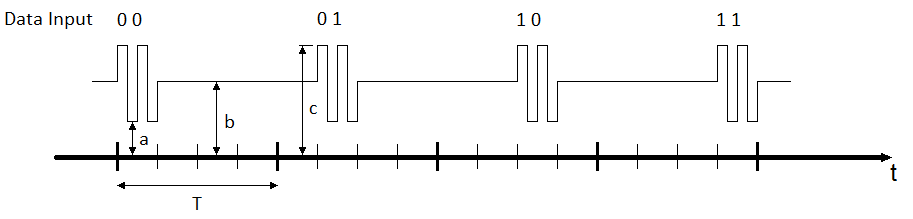
\includegraphics[width=\textwidth]{./Figures/slide0042_image022.png}
	\caption{Brithness control using sub-carrier modulation}
	\label{fig:carrier_depth}
\end{figure}

There is also one other joint brightness control and data transmission method proposed in the same paper \cite{sugiyama2007brightness}. It employs PWM modulation of the subcarrier signal to set the average value of the PPM signal. This approach provides limited brightness control in the range 0\% to 87.5\%. Additional low pass filter is required at receiver end to get rid of the overriding PWM signal.

Both of these approaches have short comings in digital systems due to use of higher frequency switching pulses as compared to the data transmission rate. Moreover the underlying brightness control circuitry needs analogue hardware. However the presence of subcarrier provides better noise immunity to external noise such as other light sources' flickering with an associated deficit that much of the device bandwidth is lost to this higher frequency carrier. Therefore these schemes are useful only for low speed data transmission.

A recent research \cite{bai2010joint} proposes the use of overlapping pulse position modulation (OPPM) for simultaneous brightness control and data transmission.  OPPM allows the pulses in adjacent slots to overlap. The constant duty cycle signal is then amplitude modulated to achieve brightness control. This scheme, too, achieves brightness control through drive current intensity control that renders it not a preferred choice for digital systems.

%One more publication \cite{sugiyama2006experimental} considers both the communication and brightness aspects of led lights, proposes methods such as inverted pulse position modulation and subcarrier inverted pulse position modulation to achieve the two objectives simultaneously. However it emphasises more on rejecting the background light flickering noise.

